\documentclass[12pt]{exam}

% essential packages
\usepackage{fullpage} % margin formatting
\usepackage{enumitem} % configure enumerate and itemize
\usepackage{amsmath, amsfonts, amssymb, mathtools} % math symbols
\usepackage{xcolor, colortbl} % colors, including in tables
\usepackage{makecell} % thicker \Xhline in table
\usepackage{graphicx} % images, resizing

% sometimes needed packages
\usepackage{hyperref} % hyperlinks
% \hypersetup{colorlinks=true, urlcolor=blue}
% \usepackage{logicproof} % natural deduction
\usepackage{tikz} % drawing graphs
\usetikzlibrary{positioning}
\usepackage{multicol}
% \usepackage{algpseudocode} % pseudocode

% paragraph formatting
\setlength{\parskip}{6pt}
\setlength{\parindent}{ 0cm}

% newline after Solution:
\renewcommand{\solutiontitle}{\noindent\textbf{Solution:}\par\noindent}

% less space before itemize/enumerate
\setlist{topsep=0pt}

% creates \filcl to grey out cells for groupwork grading
\newcommand{\filcl}{\cellcolor{gray!25}}

% creates \probnum to get the problem number
\newcounter{probnumcount}
\setcounter{probnumcount}{1}
\newcommand{\probnum}{\arabic{probnumcount}. \addtocounter{probnumcount}{1}}

% use roman numerals by default
\setlist[enumerate]{label={(\roman*)}}

% creates custom list environments for grading guidelines, question parts
\newlist{guidelines}{itemize}{1}
\setlist[guidelines]{label={}, left=0pt .. \parindent, nosep}
\newlist{gwguidelines}{enumerate}{1}
\setlist[gwguidelines]{label={(\roman*)}, nosep}
\newlist{qparts}{enumerate}{2}
\setlist[qparts]{label={(\alph*)}}
\newlist{qsubparts}{enumerate}{2}
\setlist[qsubparts]{label={(\roman*)}}
\newlist{stmts}{enumerate}{1}
\setlist[stmts]{label={(\roman*)}, nosep}
\newlist{pflist}{itemize}{4}
\setlist[pflist]{label={$\bullet$}, nosep}
\newlist{enumpflist}{enumerate}{4}
\setlist[enumpflist]{label={(\arabic*)}, nosep}

\printanswers

\newcommand{\prevhwnum}{9}
\newcommand{\hwnum}{10}

\begin{document}
%%%%%%%%%%%%%%% TITLE PAGE %%%%%%%%%%%%%%%
\title{EECS 203: Discrete Mathematics\\
  Winter 2024\\
  Homework \hwnum{}}
\date{}
\author{}
\maketitle
\vspace{-50pt}
\begin{center}
  \huge Due \textbf{Thursday, April 18}, 10:00 pm\\
\Large No late homework accepted past midnight.\\
\vspace{10pt}

\large Number of Problems: $8+2$
\hspace{3cm}
Total Points: $100+35$
\end{center}
\vspace{25pt}
\begin{itemize}
    \item \textbf{Match your pages!} Your submission time is when you upload the file, so the time you take to match pages doesn't count against you.
    \item Submit this assignment (and any regrade requests later) on Gradescope. 
    \item Justify your answers and show your work (unless a question says otherwise).
    \item By submitting this homework, you agree that you are in compliance with the Engineering Honor Code and the Course Policies for 203, and that you are submitting your own work.
    \item Check the syllabus for full details.
\end{itemize}
\newpage
%%%%%%%%%%%%%%% TITLE PAGE %%%%%%%%%%%%%%% 

\section*{Individual Portion}
\subsection*{\probnum Color Conundrum [14 points]}
Each day Donovan Edwards either wears a T-shirt or a tank top. On a given day, there is a $70\%$ chance he wears a T-shirt and a $30\%$ chance he wears a tank top. If he wears a T-shirt, he randomly picks one of 4 pink T-shirts, 3 blue T-shirts, and 2 black T-shirts (he is equally likely to pick any particular shirt). If he wears a tank top, he randomly picks one of 2 pink tank tops, 3 white tank tops, or 2 blue tank tops.

\begin{qparts}
    \item What is the probability that he is wearing pink or white on a given day?
    \item Given that Donovan is wearing pink or white on a given day, what is the probability that he is wearing a T-shirt?
\end{qparts}

You \textbf{do not} need to simplify your answers.

\begin{solution}
\begin{qparts}
    \item Let $E$ be the event that his shirt is pink or white, $S$ be the event that he wears a T-shirt, and $T$ be the event that he wears a tank top. Then by the law of total probability
    \begin{align*}
        P(E)&=P(E\cap S) + P(E\cap T) \tag{$S\cap T=\emptyset$} \\
        &=P(E\mid S)P(S) + P(E\mid T)P(T).
    \end{align*}
    The probably that his shirt is pink or white given he wears a T-shirt is $\frac 49,$ and the probability that it is pink or white given he wears a tank top is $\frac 57.$ So the total probability is
    $$P(E)=\frac 49(0.7) + \frac 57(0.3)=\frac{331}{630}\approx 0.5253968.$$

    \item The quantity we're looking for is $P(S\mid E).$ By Bayes' theorem,
    $$P(S\mid E)=\frac{P(E\mid S)P(S)}{P(E)}.$$
    We know from the problem statement that $P(S)=0.7.$ From part (a), we know $P(E\mid S)=\frac 49$ and $P(E)=\frac{331}{630}.$ So plugging this in we get
    $$P(S\mid E)=\frac{\frac 49 \cdot 0.7}{\frac{331}{630}} = \frac{196}{331} \approx 0.5921450.$$
\end{qparts}


\textbf{Draft Grading Guidelines [14 points]}

\textbf{Part a:}
\begin{guidelines}
    \item +2 identifies that law of total probability can be used
    \item +2 correct probability for $P(E\mid S)$
    \item +2 correct probability for $P(E\mid T)$
    \item +2 correct final answer
\end{guidelines}
\textbf{Part b:}
\begin{guidelines}
    \item +2 identifies that Bayes' theorem can be used
    \item +2 substitutes in correct values
    \item +2 correct final answer
\end{guidelines}
\end{solution}

\subsection*{\probnum Bayes' $\times 3$ [8 points]}
Suppose that $E$, $F_1$, $F_2$, and $F_3$ are events from a sample space $S.$ Furthermore, suppose that $F_1$, $F_2$, and $F_3$ are each mutually exclusive, and that their union is $S$. Find $P(F_2 \mid E)$ if
\begin{align*}
    P(E \mid F_2) &= \frac 38 & P(F_1) &= \frac 16 \\
    P(E \mid F_3) &= \frac 12 & P(F_2) &= \frac 12 \\
    P(E \mid F_1) &= \frac 27 & P(F_3) &= \frac 13
\end{align*}
Express your final answer as a \textbf{single, fully-simplified} number.

\begin{solution}
By the generalized version of Bayes' theorem,
\begin{align*}
P(F_2 \mid E) &= \frac{P(E \mid F_2)P(F_2)}{P(E \mid F_1)P(F_1) + P(E \mid F_2)P(F_2) + P(E \mid F_3)P(F_3)} \\
&= \frac{\frac 38\cdot\frac 12}{\frac 27\cdot\frac 16 + \frac 38\cdot\frac 12 + \frac 12\cdot\frac 13} \\
&= \frac{7}{15}.
\end{align*}

\textbf{Draft Grading Guidelines [8 points]}
\begin{guidelines}
    \item +4 select correct form of Bayes' theorem
    \item +4 correct final answer
\end{guidelines}
\end{solution}

\subsection*{\probnum There Snow Way I'm Running In This [12 points] }
Ishaan likes to run, but he hates running in the snow. If it snows, the probability of Ishaan going for a run is $\frac 1{10}$. If it doesn't snow, the probability of Ishaan running is $\frac 8{10}$. If Ishaan goes for run, then the probability that it snowed is $\frac 19.$ What is the probability that it snows?

Express your final answer as a \textbf{single, fully-simplified} number.

\begin{solution}
Let $S$ be the event that it snowed, and $R$ be the event that Ishaan runs. We are given $P(R\mid S)=\frac{1}{10},$ $P(R\mid \overline{S})=\frac 8{10},$ and $P(S\mid R)=\frac 19.$ By Bayes' theorem, we know
$$P(S\mid R) = \frac{P(R\mid S)P(S)}{P(R\mid S)P(S) + P(R\mid \overline{S})P(\overline{S})}$$
which implies
$$P(S\mid R)\left(P(R\mid S)P(S) + P(R\mid \overline{S})P(\overline{S})\right)=P(R\mid S)P(S).$$
We can substitute $P(\overline{S})=1-P(S),$ as well as the values we know to get
$$\frac 19 \left(\frac 1{10}P(S) + \frac 8{10}(1-P(S))\right)=\frac 1{10}P(S).$$
Combining like terms and solving for $P(S),$ we get
$$P(S)=\frac 12.$$

\textbf{Draft Grading Guidelines [12 points]}
\begin{guidelines}
    \item +2 correctly identifies $P(R\mid S)$
    \item +2 correctly identifies $P(R\mid \overline{S})$
    \item +2 correctly identifies $P(S\mid R)$
    \item +2 attempts to solve for $P(S)$
    \item +2 applies correct form of Bayes' theorem
    \item +2 correct final answer
\end{guidelines}
\end{solution}

\newpage

\subsection*{\probnum What did you expect? [12 points]}

The EECS 203 staff is going on a road trip! The 36 staff members have decided to split up into 6 different cars with 9, 8, 6, 6, 4, 3 people in each of the respective cars. 
\begin{qparts}
    \item Suppose we pick a car uniformly at random, and consider $X$ to be the random variable defined by the number of staff members in that car. What is the expected value of $X$?
    \item Now suppose we pick one of the staff members uniformly at random. Let $Y$ be the random variable defined by the number of people in the car that staff member is in. What is the expected value of $Y$?
\end{qparts}
Express your final answers as \textbf{single, fully-simplified} numbers.

\begin{solution}
\begin{qparts}
    \item In this case each car is equally likely to be chosen with probability $\frac 16.$ So
    \[E(X) = \frac 16(9 + 8 + 6 + 6 + 4 + 3) = 6.\]
    
    \item With this set up it is no longer equally likely for each car to be chosen. So
    \begin{align*}
        E(Y) &= 3 \cdot P(Y=3) + 4\cdot P(Y=4) + 6 \cdot P(Y=6) + 8 \cdot P(Y = 8) + 9 \cdot P(Y = 9) \\
        &= 3\cdot\frac{3}{36}+4\cdot\frac{4}{36}+6\cdot\frac{12}{36}+8\cdot\frac{8}{36}+9\cdot\frac{9}{36} \\
        &= \frac{121}{18} \approx 6.722.
    \end{align*}
\end{qparts}

\textbf{Draft Grading Guidelines [12 points]}

\textbf{Part a:}
\begin{guidelines}
    \item +2 correct expected value
    \item +2 correct justification
\end{guidelines}
\textbf{Part b:}
\begin{guidelines}
    \item +2 identifies the rooms have different probabilities of being selected
    \item +2 selects correct expected value formula
    \item +2 correct expected value
    \item +2 correct justification
\end{guidelines}
\end{solution}

\subsection*{\probnum Zero-sum game...or is it? [12 points]}

Your friend proposes to play the following game. You roll a fair, 6-sided dice twice and record the result. Let $X$ be the random variable defined as twice the value of the first roll, minus three times the value of the second roll. For example, if you rolled $3$ then $4,$ then $X$ would equal $2\cdot 3 - 3\cdot 4=-6.$ You win $X$ dollars if $X$ is positive, but have to give your friend $|X|$ dollars if $X$ is negative. If $X$ is zero then you neither win nor lose money. How much money do you expect to win or lose?

Express your final answer as a \textbf{single, fully-simplified} number.

\begin{solution}
Define random variables $X_1$ and $X_2$ as the number rolled on the first and second die respectively.

Then, $E(X_1) = E(X_2) = \frac{1}{6}(1+2+3+4+5+6) = \frac{7}{2}$.

By definition $X=2X_1 - 3X_2,$ so by linearity of expectation
$$E(X)=E(2X_1-3X_2)=2E(X_1)-3E(X_2)=2\cdot \frac 72 - 3\cdot \frac 72=-\frac 72.$$

Therefore, you would expect to lose $3.5$ dollars.

\textbf{Draft Grading Guidelines [12 points]}
\begin{guidelines}
    \item +3 defines random variables for each roll
    \item +2 correct expected value of a particular roll
    \item +2 correct definition of $X$ in terms of previous variables
    \item +2 applies linearity of expectation
    \item +3 correct final answer
\end{guidelines}
\end{solution}

\subsection*{\probnum Rollie Pollie [15 points]}

Rohit recently became super passionate about rolling dice. He decides to roll a single fair 6-sided die 100 times. What is the expected number of times he rolls a 5 followed by a 6?

Express your final answer as a \textbf{single, fully-simplified} number.

\begin{solution}
Since we are looking for a 5 followed by a 6, we define an experiment/trial to be two dice rolls. For example, the dice roll sequence 1, 2, 3 would produce 2 trials (1,2) and (2,3). Note that this means for 100 rolls we will have 99 trials.

Let $I_k$ be an indicator random variable for the $k$-th trial, where $I_k=1$ if the result of the $k$-th trial is (5,6), and is 0 otherwise. Let $X$ be the random variable for the total number of times a 5 followed by a 6 appears in the sequence. By this construction
$$X=\sum_{k=1}^{99} I_k.$$
Moreover we know the probability that we roll a 5 then a 6 on any pair of consecutive rolls is $\frac16\cdot \frac16 = \frac 1{36},$ so $I_k = \frac{1}{36}$ for every trial, $k$. By linearity of expectation, we have
$$E(X) = E\left(\sum_{k=1}^{99} I_k\right) = \sum_{k=1}^{99} E(I_k) = \sum_{k=1}^{99} \frac 1{36} = \frac{99}{36} = \frac{11}{4}.$$

\textbf{Grading Guidelines [15 points]}
\begin{guidelines}
    \item +3 correct probability of rolling a 5 followed by a 6
    \item +4 correct number of trials (99)
    \item +4 attempts to apply linearity of expectation
    \item +4 correct final answer
\end{guidelines}
\end{solution}

\subsection* {\probnum Bernoulli trials, binomial distribution [15 points]}

You roll a fair six-sided die 12 times. Find:
\begin{qparts}
    \item The probability that exactly two rolls come up as a 6.
    \item The probability that exactly two rolls come up as a 6, given that the first four rolls each came up as 3.
    \item The probability that at least two rolls come up as a 6.
    \item The expected number of rolls that come up as 6.
\end{qparts}

You \textbf{do not} need to simplify your answers.

\begin{solution}
\begin{qparts}
    \item We apply the formula for a binomial distribution with $p = \frac{1}{6}$, $n = 12$, and $k=2$. If $X$ is the number of rolls that come up as a 6: $P(X = 2) = \binom{12}{2}(\frac{1}{6})^2(\frac{5}{6})^{10}$
    
    \item Since these events are independent, then the first four rolls being determined reduces to the previous problem, but with $n=8$, so $P(X = 2) = \binom{8}{2}(\frac{1}{6})^2(\frac{5}{6})^6$
    
    \item We can find the probability that less than two rolls come up as 6, and subtract that from 1:
    \begin{align*}
        P(X \geq 2) &= 1 - (P(X = 0) + P(X = 1)) \\
        &= 1-\left[\binom{12}{0}\left(\frac{1}{6}\right)^0\left(\frac{5}{6}\right)^{12} + \binom{12}{1}\left(\frac{1}{6}\right)^1\left(\frac{5}{6}\right)^{11}\right] \\
        &= 1-\left[\left(\frac{5}{6}\right)^{12} + 12\left(\frac{1}{6}\right)\left(\frac{5}{6}\right)^{11}\right]
    \end{align*}

    \item We can apply the formula for expected value of a binomial with $p = \frac{1}{6}$ and $n = 12$. Then $E(X) = np = 12 (\frac{1}{6}) = 2$.
\end{qparts}

\textbf{Draft Grading Guidelines [15 points]}

\textbf{Parts a, b, d:}
\begin{guidelines}
    \item +2 identifies correct parameters for binomial distribution
    \item +1 correct answer
\end{guidelines}
\textbf{Part c:}
\begin{guidelines}
    \item +2 uses difference rule
    \item +1 correct expression for $P(X=0)$
    \item +1 correct expression for $P(X=1)$
    \item +2 correct answer
\end{guidelines}
\end{solution}

\subsection*{\probnum Fastest Draw in the Midwest [12 points]}

Suppose Grace has a standard deck of 52 cards. Grace expects she can draw all 52 cards in order (defined below) in 1300 draws. Yunsoo expects 1600 draws. Explain why Yunsoo is further away from the real expected value.

\textbf{Note:} The order of cards goes Ace, 2, 3, $\dots$, King and $\clubsuit, \diamondsuit, \heartsuit , \spadesuit$. If the next card in order is not drawn, then it is placed back into the deck at random. If the next card in order is drawn, then Grace sets it aside, removing it from the deck.

\textbf{Note:} The cards do not have to be selected consecutively. For example, \underline{A$\clubsuit$}, $3\diamondsuit,$ J$\spadesuit,$ \underline{2$\clubsuit$} is a valid start, and there would only be 50 cards left in the deck at this point.

\begin{solution}
We can use linearity of expectations to find the number of expected number of cards that Grace must draw.

The first card (A$\clubsuit$) has a probability of $\frac{1}{52}$ of being drawn, so the expected value is 52 draws. Since the card will not be replaced, the next card (2$\clubsuit$), has a probability of $\frac{1}{51}$ of being drawn and the expected value of 51 draws. Since the number of tries until Grace draws a particular card follows a geometric distribution, in expectation it takes her 52 tries to draw A$\clubsuit$, 51 tries to draw $2\clubsuit,$ etc.

With this pattern, it takes
$$52 + 51 + \dots + 2 + 1 = \sum_{k=1}^{52} k = \frac{52\cdot 53}2 = 1378$$
draws in expectation. So Grace's guess of 1300 draws was closer than Yunsoo's guess of 1600.

\textbf{Draft Grading Guidelines [12 points]}
\begin{guidelines}
    \item +3 identifies the use of a geometric distribution
    \item +3 correct expectation of a particular trial
    \item +3 applies linearity of expectation
    \item +3 correct final answer
\end{guidelines}
\end{solution}

\pagebreak
\section*{Grading of Groupwork \prevhwnum{}}
Using the solutions and Grading Guidelines, grade your Groupwork \prevhwnum{} Problems:
\begin{itemize}
    \item Use the table below to grade your past groupwork submission and calculate scores.
    \item While grading, mark up your past submission. Include this with the table when you submit your grading.
    \item Write whether your submission achieved each rubric item. If it didn't achieve one, say why not.
    \item For extra credit, write positive comment(s) about your work.
    \item You don't have to redo problems correctly, but it is recommended!
    \item See ``All About Groupwork" on Canvas for more detailed guidance, and what to do if you change groups.
\end{itemize}

\begin{center}
\resizebox{\textwidth}{!}{\begin{tabular}{| c | c | c | c | c | c | c | c | c | c | c | c | c |}
\hline
 & (i) & (ii) & (iii) & (iv) & (v) & (vi) & (vii) & (viii) & (ix) & (x) & (xi) & Total:\\
\hline
Problem 1 & & & & & &\filcl &\filcl &\filcl &\filcl & \filcl& \filcl& \hspace{1cm}/15\\
\hline 
Problem 2 & & & & & & & & &\filcl & \filcl& \filcl& \hspace{1cm}/15\\
\Xhline{1.25pt}
Total: &\filcl &\filcl &\filcl &\filcl &\filcl &\filcl &\filcl &\filcl & \filcl& \filcl& \filcl&\hspace{1cm}/30\\
\hline
\end{tabular}}
\end{center}

\pagebreak
\setcounter{probnumcount}{1}
\section*{Groupwork \hwnum{} Problems}

\subsection*{\probnum Circular Reasoning [15 points]}

Suppose we select $2n$ distinct points independently and uniformly at random on the border of a circle, and label them $p_1$ through $p_{2n}$ counter-clockwise (i.e. point $p_2$ is counter-clockwise from point $p_1$).

\begin{qparts}
    \item In the case where $n=2$, we have four distinct points on the circle. If we select two of these points uniformly at random and draw a line segment between them, then draw a line segment between the remaining two points, what is the probability that these line segments intersect?
    
    \textbf{Hint:} Consider the different cases corresponding to the point $p_1$ is paired with.
    
    \item Suppose we repeat the procedure in (a) where we select two points at random and draw a line segment between them. We'll call this line segment $\ell_1.$ We repeat this again with the $2n-2$ remaining points, creating a line segment $\ell_2$, etc., until we have drawn $n$ line segments: $\ell_1,\dots,\ell_n.$ After this procedure is completed, what is the expected number of intersections? Your answer should be in terms of $n.$
    
    \textbf{Hint:} Create an indicator random variable for each possible intersection and apply linearity of expectation.
    
    \textit{Note:} The number of intersections is the number of pairs $(\ell_i,\ell_j)$ of distinct line segments where $\ell_i$ and $\ell_j$ intersect.
\end{qparts}
\begin{solution}
    \begin{qparts}
        \item We have two line segments, $\ell_1$ and $\ell_2.$ Without loss of generality, let $p_1$ be an endpoint of $\ell_1$. Then it is equally likely that any of $p_2, p_3,$ or $p_4$ is the other endpoint. Define $\ell_2$ using the remaining points. Note that $\ell_1$ and $\ell_2$ will only intersect when $\ell_1$ is bounded by $p_1$ and $p_3$. Hence, the probability of intersection is $\frac{1}{3}$.

        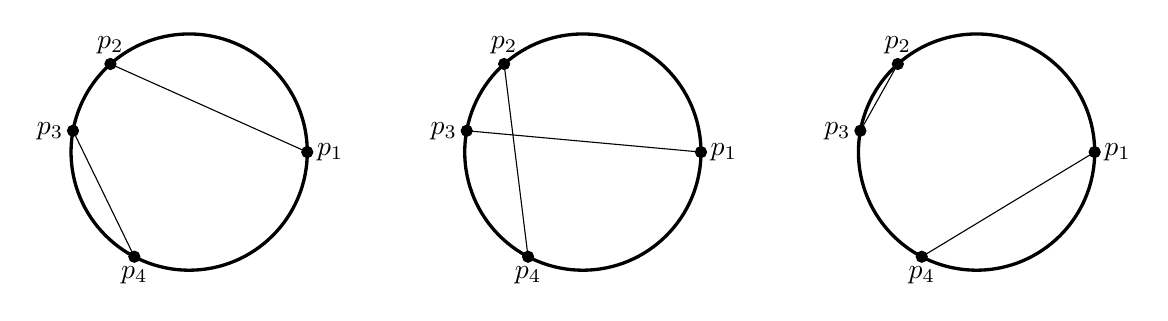
\begin{tikzpicture}
        \draw[very thick](0,0) circle (1.5);
        \filldraw[black] (1.5,0) circle (2pt) node[anchor=west]{$p_1$};
        \filldraw[black] (-1,1.119) circle (2pt) node[anchor=south]{$p_2$};
        \filldraw[black] (-1.475,0.271) circle (2pt) node[anchor=east]{$p_3$};
        \filldraw[black] (-0.696,-1.329) circle (2pt) node[anchor=north]{$p_4$};
        \draw[black] (1.5,0) -- (-1,1.119);
        \draw[black] (-1.475,0.271) -- (-0.696,-1.329);

        \draw[very thick](5,0) circle (1.5);
        \filldraw[black] (6.5,0) circle (2pt) node[anchor=west]{$p_1$};
        \filldraw[black] (4,1.119) circle (2pt) node[anchor=south]{$p_2$};
        \filldraw[black] (3.525,0.271) circle (2pt) node[anchor=east]{$p_3$};
        \filldraw[black] (4.304,-1.329) circle (2pt) node[anchor=north]{$p_4$};
        \draw[black] (6.5,0) -- (3.525,0.271);
        \draw[black] (4,1.119) -- (4.304,-1.329);

        \draw[very thick](10,0) circle (1.5);
        \filldraw[black] (11.5,0) circle (2pt) node[anchor=west]{$p_1$};
        \filldraw[black] (9,1.119) circle (2pt) node[anchor=south]{$p_2$};
        \filldraw[black] (8.525,0.271) circle (2pt) node[anchor=east]{$p_3$};
        \filldraw[black] (9.304,-1.329) circle (2pt) node[anchor=north]{$p_4$};
        \draw[black] (11.5,0) -- (9.304,-1.329);
        \draw[black] (9,1.119) -- (8.525,0.271);
        \end{tikzpicture}

        \item We first label our lines $\ell_1, \dots, \ell_n$. Let $X$ be the random variable that counts intersections between these lines. Now, define indicator random variables $X_{ij}$ for all $1 \leq i < j \leq n$ so that $X_{ij} = 1$ provided that $\ell_i$ and $\ell_j$ intersect, and $X_{ij} = 0$ otherwise. By part (a), we know that $E(X_{ij}) = \frac{1}{3}$. Moreover, since there are $\binom{n}{2}$ possible intersections between $n$ distinguishable line segments, we can use linearity of expectation to say that
        \begin{align*}
            E(X) &= E\left(\sum_{1\le i<j\le n} X_{ij}\right)\\
            &= \sum_{1\le i<j\le n} E(X_{ij})\\
            &= \binom{n}{2}\cdot\frac{1}{3}\\
            &= \frac{n!}{6(n-2)!}\\
            &= \frac{n(n - 1)}{6}.
        \end{align*}
    \end{qparts}
    
\textbf{Grading Guidelines [15 points]}

\textbf{Note:} Students are not required to simplify their answers to receive full credit.

\textbf{Part a:}
\begin{gwguidelines}
    \item +3 considers three cases, one for each possible pairing of $p_1$ (does not need to be explicit)
    \item +3 concludes that the line segments intersect in only one case, thus the probability is $\frac 13$
\end{gwguidelines}
\textbf{Part b:}
\begin{gwguidelines}[resume]
    \item +2 correct setup of indicator variables
    \item +2 recognizes that $P(X_{ij}=1)=\frac 13$ by part (a)
    \item +3 recognizes that there are $\binom{n}{2}$ indicator RVs
    \item +2 correct final answer
\end{gwguidelines}
\end{solution}

\subsection*{\probnum Open or Closed [20 points]}

\textit{Online Bayesian Inference} is a process where we repeatedly apply Bayes
rule to update our beliefs over time. Suppose we have a sensor that determines
whether a door is open or closed. 
If the door is open, the sensor reads it as open with probability 0.9. 
If the door is closed, the sensor reads it as closed with probability 0.7. Suppose the door starts in an unknown position, and has equal probability of being open or closed.

\begin{qparts}
    \item After one reading that the door is closed, what is the probability that the  door is actually closed?
    \item Before the second reading, we believe that the door is closed with the 
    probability found in part (a) (that is, we consider the probability that the door
    is closed to be the probability that we found the door is closed given our first reading). 
    Suppose we make another reading that the door  is closed. Now what is 
    the probability that the door is closed?
    \item On the third reading, the sensor reads that the door is open. What is 
    the probability that the door is actually closed, using the answer from part (b)
    as our initial probability for the door being closed?
\end{qparts}

\begin{solution}
\begin{qparts}
    \item Let $C$ be the event that the door is closed. At first, we believe $P(C) = 0.5$.
    Let $R_1$ be the event that the first reading is closed. We know $P(R_1 \mid C) = 0.7$
    and $P(R_1 \mid \overline{C}) = 1 - 0.9 = 0.1$. Then by Bayes' rule: 
    \begin{align*}
    P(C \mid R_1) &= \frac{P(R_1 \mid C) P(C)}{P(R_1 \mid C) P(C) + P(R_1 \mid \overline{C}) P(\overline{C})} \\
    &= \frac{0.7 \cdot 0.5}{0.7 \cdot 0.5 + 0.1 \cdot 0.5} \\
    &= \frac{0.35}{0.4} \\
    &= 0.875.
    \end{align*}

    \item We repeat the same process but use the updated probabilities from part (a) as 
    $P(C)$ and $P(\overline{C})$. This gives us:
    \begin{align*}
    P(C \mid R_2) &= \frac{P(R_2 \mid C) P(C)}{P(R_2 \mid C) P(C) + P(R_2 \mid \overline{C}) P(\overline{C})} \\
    &= \frac{0.7 \cdot 0.875}{0.7 \cdot 0.875 + 0.1 \cdot 0.125} \\
    &= \frac{0.6125}{0.6125 + 0.0125} \\
    &= 0.98.
    \end{align*}

    \item We use a similar process, but different probabilities. 
    \begin{align*}
    P(C \mid \overline{R_3}) &= \frac{P(\overline{R_3} \mid C) P(C)}{P(\overline{R_3} \mid C) P(C) + P(\overline{R_3} \mid \overline{C}) P(\overline{C})} \\
    &= \frac{0.3 \cdot 0.98}{0.3 \cdot 0.98 + 0.9 \cdot 0.02} \\
    &= \frac{0.294}{0.294 + 0.018} \\
    &\approx 0.94 .
    \end{align*}
\end{qparts}

\textbf{Grading Guidelines [20 points]}

\textbf{Part a:}
\begin{gwguidelines}
    \item +2 correctly identifies $P(C)$
    \item +2 correctly identifies $P(R_1\mid C)$
    \item +2 correctly identifies $P(R_1\mid \overline{C})$
    \item +2 attempts to solve for $P(C\mid R_1)$
    \item +2 correct final answer
\end{gwguidelines}
\textbf{Part b:}
\begin{gwguidelines}[resume]
    \item +2 correctly uses value from (a) for $P(C)$
    \item +2 correct final answer (based on answer from (a))
\end{gwguidelines}
\textbf{Part b:}
\begin{gwguidelines}[resume]
    \item +2 correctly uses value from (a) for $P(C)$
    \item +2 correctly identifies $P(\overline{R_3}\mid C)$ and $P(\overline{R_3}\mid \overline{C})$
    \item +2 correct final answer (based on answer from (a))
\end{gwguidelines}

\end{solution}


\end{document}
